%% March 2018
%%%%%%%%%%%%%%%%%%%%%%%%%%%%%%%%%%%%%%%%%%%%%%%%%%%%%%%%%%%%%%%%%%%%%%%%%%%%
% AGUJournalTemplate.tex: this template file is for articles formatted with LaTeX
%
% This file includes commands and instructions
% given in the order necessary to produce a final output that will
% satisfy AGU requirements, including customized APA reference formatting.
%
% You may copy this file and give it your
% article name, and enter your text.
%
%
% Step 1: Set the \documentclass
%
% There are two options for article format:
%
% PLEASE USE THE DRAFT OPTION TO SUBMIT YOUR PAPERS.
% The draft option produces double spaced output.
%

%% To submit your paper:
\documentclass[draft,linenumbers]{agujournal2018}
\usepackage{apacite}
\usepackage{url} %this package should fix any errors with URLs in refs.
%%%%%%%
% As of 2018 we recommend use of the TrackChanges package to mark revisions.
% The trackchanges package adds five new LaTeX commands:
%
%  \note[editor]{The note}
%  \annote[editor]{Text to annotate}{The note}
%  \add[editor]{Text to add}
%  \remove[editor]{Text to remove}
%  \change[editor]{Text to remove}{Text to add}
%
% complete documentation is here: http://trackchanges.sourceforge.net/
%%%%%%%


%% Enter journal name below.
%% Choose from this list of Journals:
%
% JGR: Atmospheres
% JGR: Biogeosciences
% JGR: Earth Surface
% JGR: Oceans
% JGR: Planets
% JGR: Solid Earth
% JGR: Space Physics
% Global Biogeochemical Cycles
% Geophysical Research Letters
% Paleoceanography and Paleoclimatology
% Radio Science
% Reviews of Geophysics
% Tectonics
% Space Weather
% Water Resources Research
% Geochemistry, Geophysics, Geosystems
% Journal of Advances in Modeling Earth Systems (JAMES)
% Earth's Future
% Earth and Space Science
% Geohealth
%
% ie, \journalname{Water Resources Research}

\journalname{Geochemistry, Geophysics, Geosystems}

% Pandoc citation processing
\newlength{\csllabelwidth}
\setlength{\csllabelwidth}{3em}
\newlength{\cslhangindent}
\setlength{\cslhangindent}{1.5em}
% for Pandoc 2.8 to 2.10.1
\newenvironment{cslreferences}%
  {}%
  {\par}
% For Pandoc 2.11+
\newenvironment{CSLReferences}[3] % #1 hanging-ident, #2 entry spacing
 {% don't indent paragraphs
  \setlength{\parindent}{0pt}
  % turn on hanging indent if param 1 is 1
  \ifodd #1 \everypar{\setlength{\hangindent}{\cslhangindent}}\ignorespaces\fi
  % set entry spacing
  \ifnum #2 > 0
  \setlength{\parskip}{#2\baselineskip}
  \fi
 }%
 {}
\usepackage{calc} % for calculating minipage widths
\newcommand{\CSLBlock}[1]{#1\hfill\break}
\newcommand{\CSLLeftMargin}[1]{\parbox[t]{\csllabelwidth}{#1}}
\newcommand{\CSLRightInline}[1]{\parbox[t]{\linewidth - \csllabelwidth}{#1}}
\newcommand{\CSLIndent}[1]{\hspace{\cslhangindent}#1}

\usepackage{soulutf8}
\usepackage{setspace}
\usepackage{caption}
\captionsetup[figure]{font={stretch=0.6, footnotesize}}
\usepackage{hyperref}
\usepackage{amsmath}
\usepackage{amsfonts}
\usepackage{float}
\usepackage{booktabs}
\usepackage{longtable}
\usepackage{array}
\usepackage{multirow}
\usepackage{wrapfig}
\usepackage{float}
\usepackage{colortbl}
\usepackage{pdflscape}
\usepackage{tabu}
\usepackage{threeparttable}
\usepackage{threeparttablex}
\usepackage[normalem]{ulem}
\usepackage{makecell}
\usepackage{xcolor}

\begin{document}

%% ------------------------------------------------------------------------ %%
%  Title
%
% (A title should be specific, informative, and brief. Use
% abbreviations only if they are defined in the abstract. Titles that
% start with general keywords then specific terms are optimized in
% searches)
%
%% ------------------------------------------------------------------------ %%

% Example: \title{This is a test title}

\title{A comparison of global heat flow interpolation techniques}

%% ------------------------------------------------------------------------ %%
%
%  AUTHORS AND AFFILIATIONS
%
%% ------------------------------------------------------------------------ %%

% Authors are individuals who have significantly contributed to the
% research and preparation of the article. Group authors are allowed, if
% each author in the group is separately identified in an appendix.)

% List authors by first name or initial followed by last name and
% separated by commas. Use \affil{} to number affiliations, and
% \thanks{} for author notes.
% Additional author notes should be indicated with \thanks{} (for
% example, for current addresses).

% Example: \authors{A. B. Author\affil{1}\thanks{Current address, Antartica}, B. C. Author\affil{2,3}, and D. E.
% Author\affil{3,4}\thanks{Also funded by Monsanto.}}

\authors{
Buchanan C. Kerswell
\affil{1}
Matthew J. Kohn
\affil{1}
}


% \affiliation{1}{First Affiliation}
% \affiliation{2}{Second Affiliation}
% \affiliation{3}{Third Affiliation}
% \affiliation{4}{Fourth Affiliation}

\affiliation{1}{Department of Geosicences, Boise State University,
Boise, ID 83725}
%(repeat as many times as is necessary)

%% Corresponding Author:
% Corresponding author mailing address and e-mail address:

% (include name and email addresses of the corresponding author.  More
% than one corresponding author is allowed in this LaTeX file and for
% publication; but only one corresponding author is allowed in our
% editorial system.)

% Example: \correspondingauthor{First and Last Name}{email@address.edu}
\correspondingauthor{Buchanan C.
Kerswell}{buchanankerswell@u.boisestate.edu}

%% Keypoints, final entry on title page.

%  List up to three key points (at least one is required)
%  Key Points summarize the main points and conclusions of the article
%  Each must be 100 characters or less with no special characters or punctuation

% Example:
% \begin{keypoints}
% \item	List up to three key points (at least one is required)
% \item	Key Points summarize the main points and conclusions of the article
% \item	Each must be 100 characters or less with no special characters or punctuation
% \end{keypoints}

\begin{keypoints}
\item 
\item 
\item 
\end{keypoints}

%% ------------------------------------------------------------------------ %%
%
%  ABSTRACT
%
% A good abstract will begin with a short description of the problem
% being addressed, briefly describe the new data or analyses, then
% briefly states the main conclusion(s) and how they are supported and
% uncertainties.
%% ------------------------------------------------------------------------ %%

%% \begin{abstract} starts the second page

\begin{abstract}

\end{abstract}
\section{Introduction}

Heat escaping the solid Earth's surface indicates a dynamically cooling
planet. Surface heat flow databases (Hasterok \& Chapman, 2008;
Lucazeau, 2019; Pollack et al., 1993) provide a way to understand
geodynamics by relating the amount of heat escaping Earth's surface to
heat-transferring and heat-generating subsurface processes such as
diffusion, hydrothermal circulation, radioactive decay, fault motion,
subduction dynamics, and mantle convection (Currie et al., 2004; Currie
\& Hyndman, 2006; Fourier, 1827; Furlong \& Chapman, 2013; Furukawa,
1993; Gao \& Wang, 2014; Hasterok, 2013; Kerswell et al., 2020; Parsons
\& Sclater, 1977; Pollack \& Chapman, 1977; Rudnick et al., 1998; Stein
\& Stein, 1992, 1994; Wada \& Wang, 2009). Surface heat flow
observations continue to motivate research, evident by more than 1,393
publications compiled in the most recent heat flow dataset, although the
rate of publications using surface heat flow has declined since the mid
1980's (Jennings \& Hasterok, 2021).

Many research questions, such as calculating the global surface heat
flux from continents and oceans, require interpolating discrete heat
flow observations onto a continuous approximation of Earth's surface.
Previous attempts at interpolation use one or more geographic, geologic,
geochronologic, or geophysical proxies to predict heat flow at unknown
locations by association with similar observation sites (e.g.,
bathymetry or elevation, proximity to active or ancient orogens,
seafloor age, upper mantle shear wave velocities, Chapman \& Pollack,
1975; Davies, 2013; Goutorbe et al., 2011; Lee \& Uyeda, 1965; Lucazeau,
2019; Sclater \& Francheteau, 1970; Shapiro \& Ritzwoller, 2004). These
methods are called \emph{similarity methods} (Figure~\ref{fig:lucahf}).
The success of such interpolations are typically evaluated statistically
by the misfit between the predicted and observed heat flow. However,
even statistically-successful heat flow interpolations are difficult to
interpret and show unexpected anomalies (Lucazeau, 2019). The fidelity
and usefulness of interpolations depend on the question being asked and
the choice of methodology.

\begin{figure}[h]

{\centering 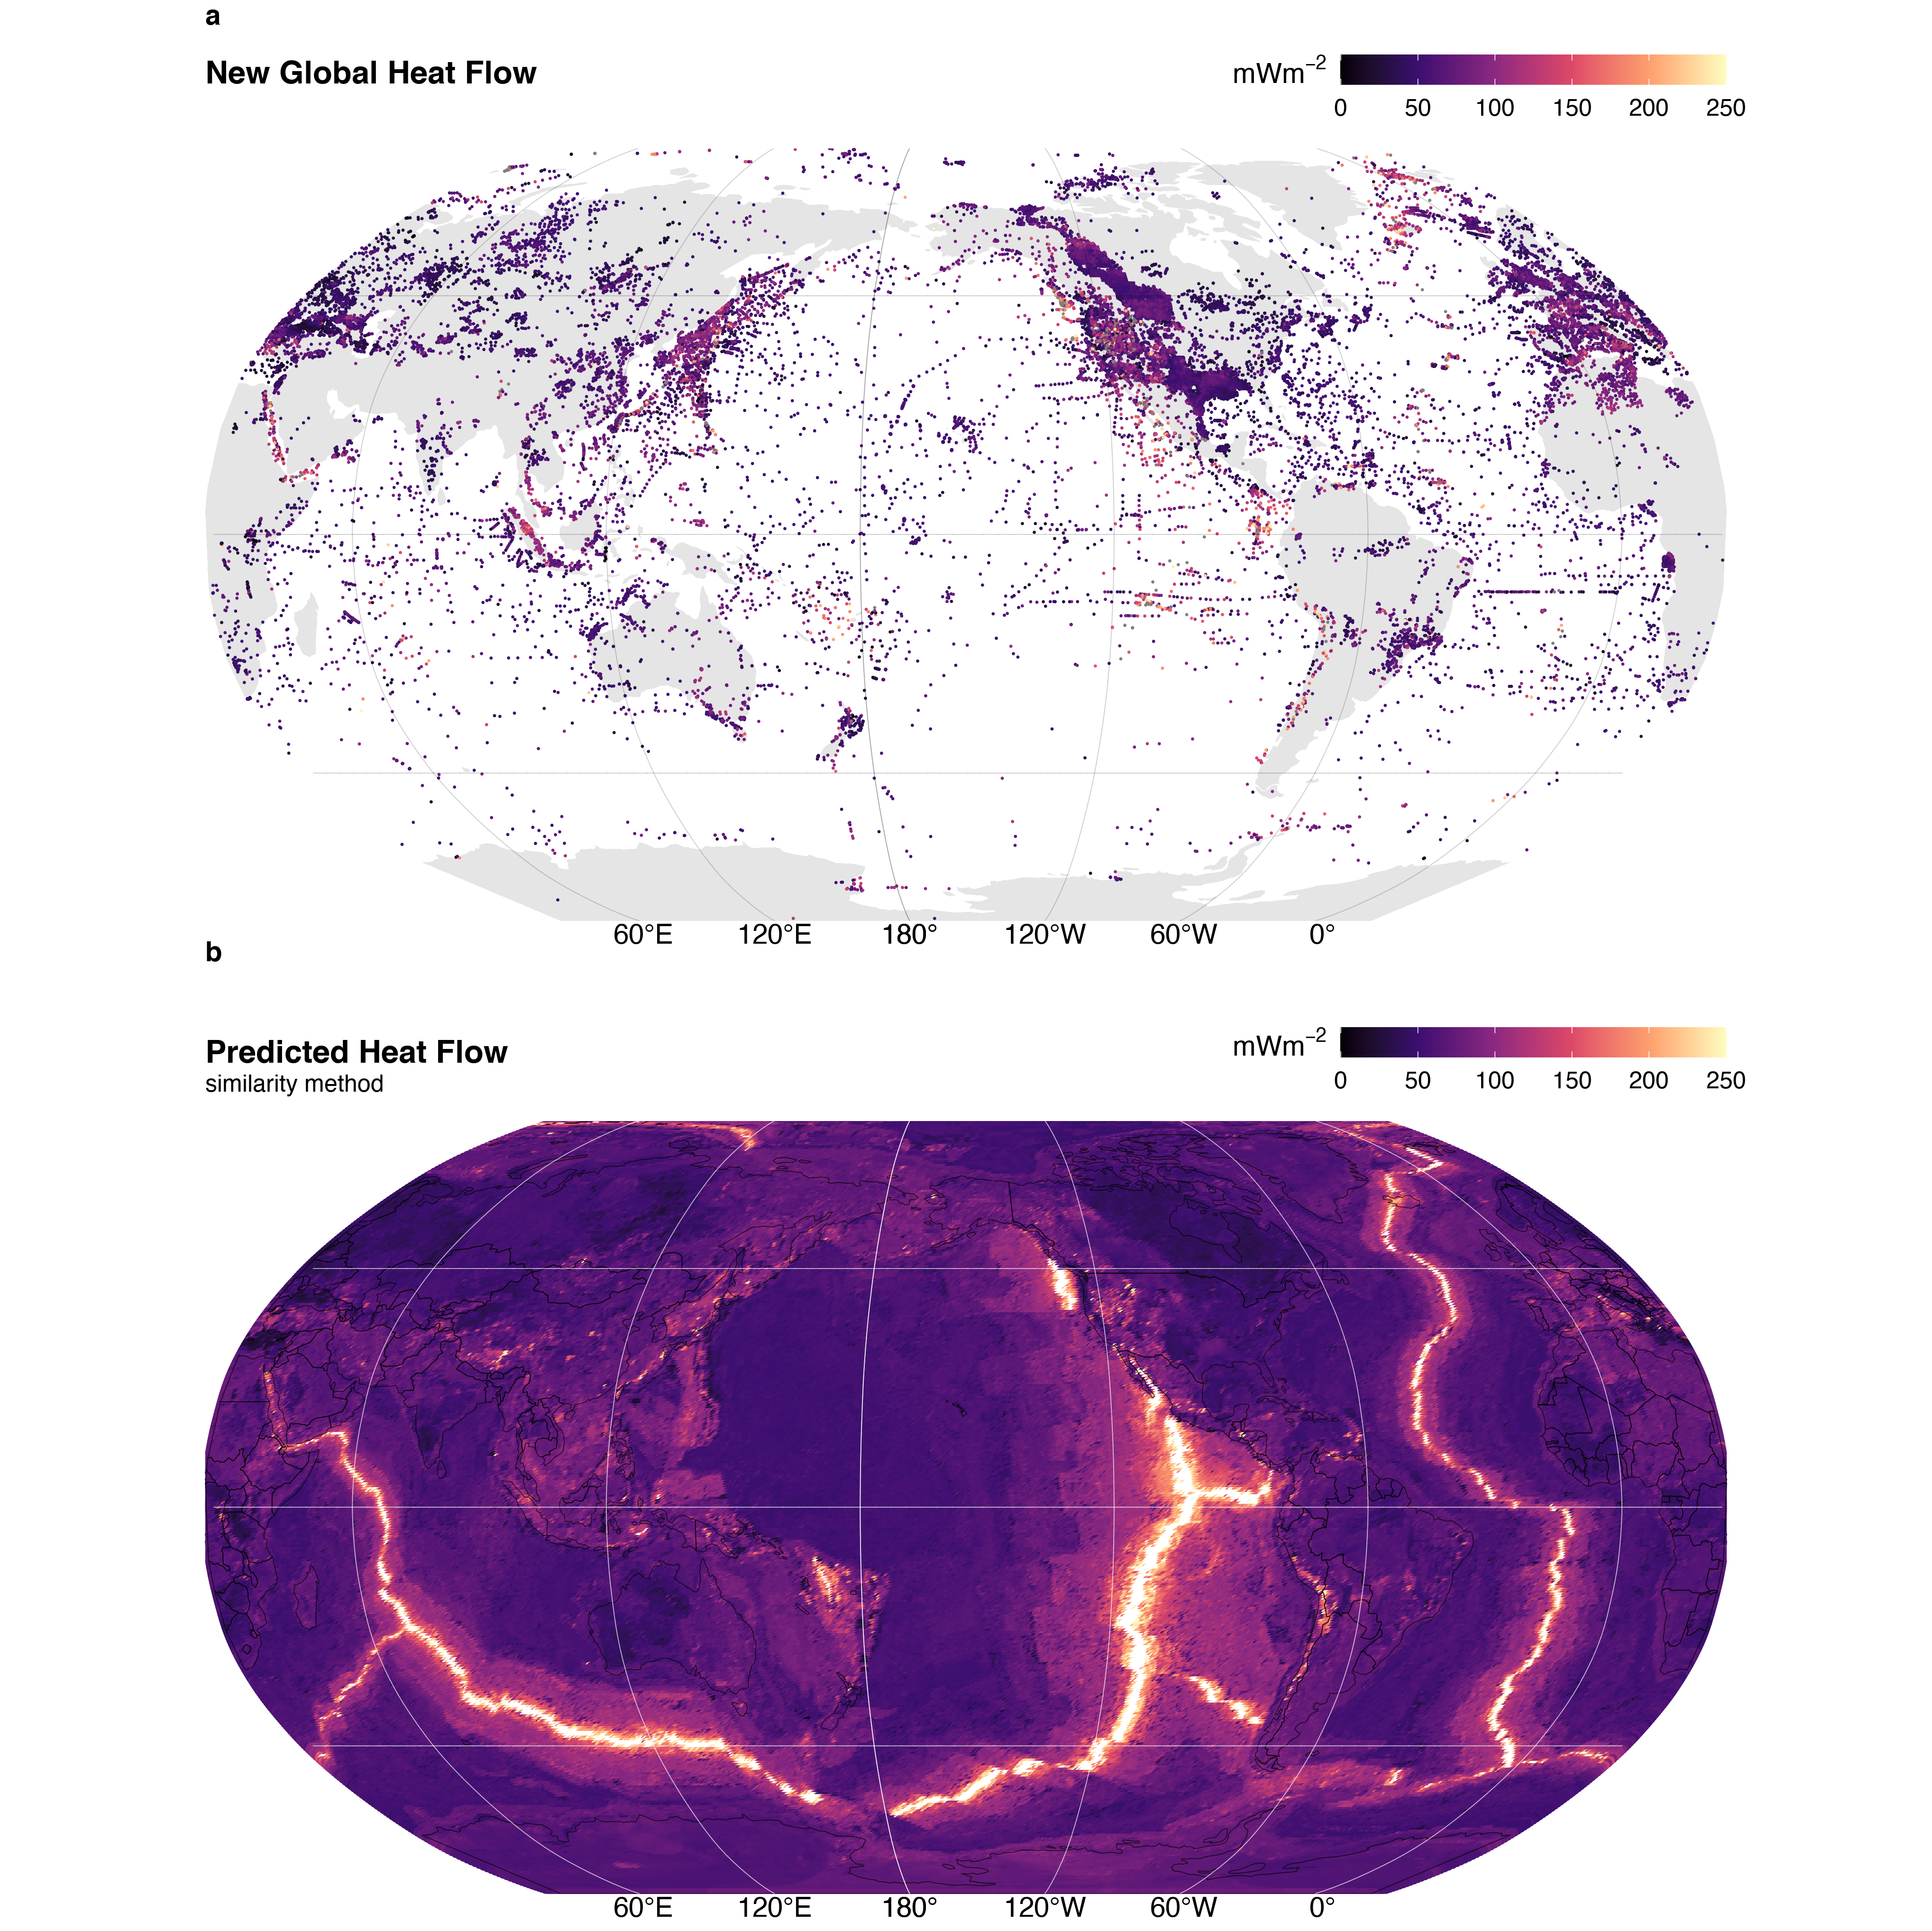
\includegraphics[width=1\linewidth,]{../figs/base/hf_luca} 

}

\caption{The NGHF dataset. (a) The complete dataset (n = 69729), and (b) interpolation by similarity method from Lucazeau (2019).}\label{fig:lucahf}
\end{figure}

Predicting surface heat flow by association with physical proxies is
arguably the most reasonable approach to interpolation for global
investigations. Our understanding of geodynamics and near-surface heat
flow perturbations implies that the variance in surface heat flow is not
uniformly stochastic, but rather, in large part, determined by the
physical conditions and processes operating locally (e.g., Goutorbe et
al., 2011). For example, younger oceanic plates should have higher
surface heat flow than older plates (Stein \& Stein, 1992), subducting
oceanic plates will lower surface heat flow near trenches (Furukawa,
1993), and hydrothermal circulation of seawater can modify heat flow in
oceanic crust (Hasterok et al., 2011). Interpolation by association with
physical proxies makes reasoned predictions of heat flow based on many
independently-tested geodynamic models. However, similarity methods are
strongly biased towards such models and risk making determinations
where, in fact, surprising results and idiosyncrasies may be found.

In contrast, there exists some degree of stationarity, spatial
dependence, or continuity, in the distribution of surface heat flow. A
pair of surface heat flow observations taken one meter apart will be
strongly correlated. The correlation between pairs of observations will
likely decrease with increasing distance between the pairs (Goovaerts,
1997). The spatial (dis)continuity of surface heat flow represents the
areal extent of geodynamic processes and their interactions. For
example, consistent patterns of heat flow near volcanic arcs are
interpreted to reflect common backarc lithospheric thermal structures
and slab-mantle mechanical coupling depths in subduction zones
(Furukawa, 1993; Kerswell et al., 2020; Wada \& Wang, 2009).

In theory, one may predict surface heat flow at unknown locations by
considering many nearby observations (i.e.~Kriging, Krige, 1951).
However, Kriging is disadvantageous for global interpolations of surface
heat flow because it assumes that the underlying distribution of heat
flow is stationary (constant in space), which effectively ignores
geodynamic complexity. One can overcome this problem by relaxing
assumptions of stationarity, or applying Markov-Bayes techniques to
include proxies as priors (Bárdossy, 1997). Instead, we leverage the
properties of stationarity as a tool for comparison with
\emph{similarity} methods of interpolation (Goutorbe et al., 2011;
Lucazeau, 2019). So the questions are: 1) What are the differences
between Kriging and similarity methods? 2) What are the implications of
the differences according to the implicit assumptions in both methods?

We attempt to answer these questions by using ordinary Kriging to
interpolate the New Global Heat Flow (NGHF) dataset of Lucazeau (2019).
Our method is optimized using a genetic algorithm to minimize an
objective function which considers both the misfit on the variogram
models and interpolation results (after Li et al., 2018). We then
compare our interpolation results to those of Lucazeau (2019) and
consider the implications of Kriging vs.~similarity methods of
interpolation. We restrict our comparison to areas near subduction zone
segments defined by Syracuse \& Abers (2006) for two reasons: 1) to
provide maps and statistics useful to subduction zone research, and 2)
to emphasize differences and idiosyncrasies in both interpolation
approaches in a complex tectonic and thermal setting.

\section{Methods}

\subsection{The NGHF Dataset}

The NGHF dataset was downloaded from the supplementary material of
Lucazeau (2019). It contains 69729 data points, their locations in
latitude/longitude, and metadata---including a data quality rank (Code
6) from A to D (with Code 6 = Z = undetermined). The reader is referred
to Lucazeau (2019) for details on compilation, references, and
historical perspective on the NGHF and previous compilations. We use
NGFH because it is the most recent dataset available, has been carefully
compiled, and is open-access.

Like Lucazeau (2019), we exclude 4790 poor quality observations (Code 6
= D) from our analysis. We further remove 350 data points without heat
flow observations and two without geographic information. Multiple
observations at the same location are parsed to avoid singular
covariance matrices during Kriging:

\begin{equation}\protect\hypertarget{eq:parse}{}{\begin{aligned}
    f(X_i^q, Y_i^q) &= \\
    X_i^q > Y_i^q &\rightarrow z_i = x_i \\
    X_i^q < Y_i^q &\rightarrow z_i = y_i \\
    X_i^q = Y_i^q &\rightarrow z_i = RAND(x_i, y_i)
    \end{aligned}}\label{eq:parse}\end{equation}

where \(X_i^q\) and \(Y_i^q\) represent the quality of each duplicate
observation pair at location \(i\), \(RAND\) is a random function that
selects either the observation \(x_i\) or \(y_i\), and \(z_i\) stores
the observation selected by \(f(X_i^q, Y_i^q)\). The final dataset used
for Kriging has \(n=\) 55274 observations after parsing \(n=\) 32430
duplicate observation.

\subsection{Kriging}

Kriging is a three-step process that involves first estimating an
experimental variogram, \(\hat{\gamma}(h)\), fitting the experimental
variogram with one of many variogram models, \(\gamma(h)\), and finally
using the modelled variogram to predict random variables at unknown
locations (Cressie, 2015; Krige, 1951). We use the general-purpose
functions defined in the ``R'' package \texttt{gstat} (Gräler et al.,
2016; Pebesma, 2004) to perform all three steps. We begin by estimating
an experimental variogram as defined by Bárdossy (1997):

\begin{equation}\protect\hypertarget{eq:variogram}{}{\hat{\gamma}(h) = \frac{1}{2N(h)}\sum_{N(h)}^{}(Z(u_i) - Z(u_j))^2}\label{eq:variogram}\end{equation}

where \(N(h)\) is the number of pairs of points, \(Z(u_i)\) and
\(Z(u_j)\), separated by a lag distance, \(h = |u_i - u_j|\). We
evaluate \(\hat{\gamma}(h)\) at fifteen lag distances by binning the
irregular spaced data with a bin width, \(\delta\), equal to one-third
of the maximum lag distance divided by the number of lags used to
evaluate the variogram, \(\delta = \max (N(h))/(3\cdot 15)\). Then
\(N(h) \leftarrow N(h, \delta h) = \{i,j:|u_i - u_j| \in [h - \delta h, h + \delta h)\}\).
In simple terms, Equation~\ref{eq:variogram} represents the similarity,
or dissimilarity, between pairs of observations in space.
Equation~\ref{eq:variogram} is derived from the theory of
\emph{regionalized variables} (Matheron, 1963, 2019), which formally
defines a probabilistic framework for spatial interpolation of natural
phenomena. It is important for the reader to understand the fundamental
assumptions implicit in Equation~\ref{eq:variogram} in order to
understand the comparison of interpolation techniques discussed later.
The basic assumptions used in our Kriging method are:

\begin{itemize}
\item
  \(\hat{\gamma}(h)\) is directionally invariant (isotropic)
\item
  \(\hat{\gamma}(h)\) is evaluated in two-dimensions and neglects
  elevation, \(Z(u) \in \mathbb{R}^2\)
\item
  The first and second moments of \(Z(u)\) have the following conditions
  over the domain \(D\):

  \begin{equation}\protect\hypertarget{eq:assumptions}{}{\begin{aligned}
        &E[Z(u)] = mean = constant, &\forall u \in D \\
        &E[(Z(u + h) - mean)(Z(u) - mean)] = C(h), &\forall |u, u + h| \in D
        \end{aligned}}\label{eq:assumptions}\end{equation}
\end{itemize}

The last assumption (Equation~\ref{eq:assumptions}) is called
``second-order stationarity'' and is commonly used in practice. It
assumes the underlying probability distribution of the random variable,
\(Z(u)\), does not change in space and the covariance, \(C(h)\), only
depends on the distance, \(h\), between two random variables. These
assumptions are expected to be valid in cases where the underlying
natural process is stochastic, spatially continuous, and has the
property of additivity such that \(\frac{1}{n}\sum_{i=1}^n Z(u_i)\) has
the same meaning as \(Z(u)\) (Bárdossy, 1997).

The following are two illustrative cases where
Equation~\ref{eq:assumptions} is likely valid:

\begin{enumerate}
\def\labelenumi{\arabic{enumi}.}
\item
  The thickness of a sedimentary unit with a homogeneous concentration
  of radioactive elements can be approximated by
  \(q_s = q_b + \int A \,dz\), where \(q_b\) is a constant heat flux
  entering the bottom of the layer and \(A\) is the heat production
  within the layer with thickness \(z\) (Furlong \& Chapman, 2013). If
  we have two samples, \(Z(u_1) = 31~mW/m^2\) and
  \(Z(u_2) = 30.5~mW/m^2\), their corresponding thicknesses would be
  \(Z'(u_1) = 1000~m\) and \(Z'(u_2) = 500~m\) for \(A = 0.001~mW/m^3\)
  and \(q_b = 30~mW/m^2\). The variable, \(Z(u)\), in this case is
  additive because the arithmetic mean of the samples is a good
  approximation of the average sedimentary layer thickness,
  \((Z(u_1) + Z(u_2)) / 2 = 750~m\).
\item
  The age of young oceanic lithosphere can be approximated by
  \(q_s(t) = kT_b(\pi\kappa t)^{-1/2}\), where \(q_s(t)\) is the surface
  heat flow of a plate with age, \(t\), \(T_b\) is the temperature at
  the base of the plate, \(k\) is thermal conductivity, and
  \(\kappa = k/\rho C_p\) is thermal diffusivity (Stein \& Stein, 1992).
  For \(k = 3.138~W/mK\), \(\rho = 3330~kg/m^3\), \(C_p = 1171~J/kgK\),
  \(T_b = 1350^{\circ}C\), two samples, \(Z(u_1) = 180~mW/m^2\) and
  \(Z(u_2) = 190~mW/m^2\), would correspond to plates with ages of
  \(Z'(u_1) = 10~Ma\), and \(Z'(u_2) = 9~Ma\), respectively. Since
  \(Z(u_1) + Z(u_2) / 2 = 185~mW/m^2\) and
  \(Z'(185~mW/m^2) = 9.5~Ma = Z'(u_1) + Z'(u_2) / 2\), the variable
  \(Z(u)\) in this case is also additive.
\end{enumerate}

In contrast, Equation~\ref{eq:assumptions} is likely invalid in regions
that transition among two or more tectonic regimes. For example, the
expected heat flow \(E[Z(u)] = mean\) will change when moving from a
spreading center to a subduction zone. \(E[Z(u)] = mean \neq constant\)
over the region of interest. Proceeding with
Equation~\ref{eq:assumptions} in this case has the effect of masking the
geodynamic complexity. In other words, the spatial dependence is
considered in the Kriging method in this case, but the geodynamic
structure is \emph{invisible}. We will see that this has important
implications when comparing our Kriging method to Lucazeau (2019)'s
interpolation method, which is exactly opposite of this formalism---it
only considers the similarities among physical proxies and not spatial
dependence.

The second step is to fit the experimental variogram with a variogram
model, \(\gamma(h)\). In this study we fit three popular variogram
models to the experimental variogram. We use models with sills, which
implies the spatial dependence between pairs of points has a finite
range. The spherical, exponential, and Guassian variogram models are
defined as (Chiles \& Delfiner, 2009; Cressie, 2015):

\begin{equation}\protect\hypertarget{eq:varmodels}{}{
\begin{aligned}
    sph &\leftarrow \gamma(h) =
        \begin{cases}
            n + s \left(\frac{3h}{2a} - \frac{1}{2}\left(\frac{h}{a}\right)^3\right), & \quad\text{if } 0 \leq h \leq a \\
            n + s, & \quad\text{if } h > a
        \end{cases} \\
    exp &\leftarrow \gamma(h) = n + s \left(1 - exp\left(\frac{-h}{a}\right)\right), ~\quad\text{if } h \geq 0 \\
    Gau &\leftarrow \gamma(h) = n + s \left(1 - exp\left(\frac{-h^2}{a^2}\right)\right), \quad\text{if } h \geq 0
\end{aligned}
}\label{eq:varmodels}\end{equation}

where \(n\) is the nugget, \(s\) is the sill, and \(a\) is the effective
range. For spherical, exponential, and Gaussian models, the effective
range is related to the range, \(r\), by \(a = r\), \(a = r/3\), and
\(a=1/r\sqrt{3}\), respectively (Gräler et al., 2016; Pebesma, 2004).
The function \texttt{fit.variogram} in \texttt{gstat} allows one to try
many variogram models and the best will be selected by the minimum
misfit by weighted least square (WLS, Pebesma, 2004).

We use ordinary Kriging for our interpolation step, which predicts the
value of a random function, \(\hat{Z}(u)\) at unknown locations as a
linear combination of all known locations in the domain, \(D\)
(Bárdossy, 1997):

\begin{equation}\protect\hypertarget{eq:linestimate}{}{ \hat{Z}(u) = \sum_{i=1}^n \lambda_i Z(u_i), \quad \forall u \in D }\label{eq:linestimate}\end{equation}

The conditions in Equation~\ref{eq:assumptions} set up a constrained
minimization problem since one has:

\begin{equation}\protect\hypertarget{eq:firstmoment}{}{ E[Z(u)] = mean, \quad \forall u \in D }\label{eq:firstmoment}\end{equation}

The linear estimator must obey

\begin{equation}\protect\hypertarget{eq:explinestimate}{}{ E[\hat{Z}(u)] = \sum_{i=1}^n \lambda_i E[Z(u_i)] = mean }\label{eq:explinestimate}\end{equation}

so the weights must be:

\begin{equation}\protect\hypertarget{eq:unbiased}{}{ \sum_{i=1}^n \lambda_i = 1 }\label{eq:unbiased}\end{equation}

This is the first constraint, also known as the unbiased condition,
which states that the sum of the weights must equal one. However, there
is an infinite set of real numbers one could use for the weights,
\(\lambda_i\). Our goal is to find the set of weights in
Equation~\ref{eq:linestimate} that minimizes the estimation variance.
This can be solved with the covariance function, \(C(h)\) from
Equation~\ref{eq:assumptions}:

\begin{equation}\protect\hypertarget{eq:minvar}{}{
\begin{aligned}
    \sigma^2(u) = Var[Z(u) - \hat{Z}(u)] = E\left[(Z(u) - \sum_{i=1}^n \lambda_i Z(u_i))^2\right] &= \\
    E\left[Z(u)^2 + \sum_{j=1}^n \sum_{i=1}^n \lambda_j \lambda_i Z(u_j)Z(u_i) - 2 \sum_{i=1}^n \lambda_i Z(u_i)Z(u)\right] &= \\
    C(0) + \sum_{j=1}^n \sum_{i=1}^n \lambda_j \lambda_i C(u_i - u_j) - 2 \sum_{i=1}^n \lambda_i C(u_i - u)
\end{aligned}
}\label{eq:minvar}\end{equation}

Solving for the weights in Equation~\ref{eq:linestimate} with respect to
the unbiased condition (Equation~\ref{eq:unbiased}) and minimum estimate
variance (Equation~\ref{eq:minvar}), yields the best linear unbiased
estimator (BLUE, Bárdossy, 1997). In our case, this is done by the
function \texttt{krige} in \texttt{gstat}.

\subsection{Kriging Optimization}

Achieving a useful Kriging results depends on one's choice of many
Kriging parameters (\(\Theta\)). In this study, we investigate a set of
parameters, \(\Theta\):

\begin{equation}\protect\hypertarget{eq:params}{}{ \Theta = \{m, s, a, n, S\} }\label{eq:params}\end{equation}

where \(m\) is the model type (sph, exp, or Gau), \(s\) is the sill,
\(a\) is the effective range, \(n\) is the nugget, and \(S\) is the
maximum distance for local Kriging. Only points within \(S\) from the
prediction location are used for Kriging. Our goal is to find \(\Theta\)
such that our interpolation, \(f(x_i; \Theta)\), gives the most useful
outcome---defined by minimizing a cost function, \(C(\Theta)\), that
represents the error between the set of real observations, \(Z(u_i)\)
and predictions, \(\hat{Z}(u)\).

We define a cost function that simultaneously considers the misfit
between the experimental and modelled variogram and between the Kriging
predictions and observed heat flow (after Li et al., 2018):

\begin{equation}\protect\hypertarget{eq:cost}{}{ C(\Theta) = (1-w)C_F(\Theta) + wC_I(\Theta) }\label{eq:cost}\end{equation}

where \(C_F(\Theta)\) is the root mean square error (RMSE) of the
modelled variogram fit calculated by WLS, and \(C_I(\Theta)\) is the
RMSE of the Kriging result calculated by cross-validation. The weight,
\(w\), is set to 0.5 in our study, which balances the effects of
\(C_F(\Theta)\) and \(C_I(\Theta)\) on the cost function. The final
expression to minimize becomes:

\begin{equation}\protect\hypertarget{eq:costexp}{}{
\begin{aligned}
    \min(C(\Theta)) =
    \frac{1-w}{\sigma_E}&\sqrt{\frac{1}{N}\sum_{k=1}^{N}w(h_k)[\hat{\gamma}(h_k)-\gamma(h_k;\Theta)]^2} \quad + \\
    \frac{w}{\sigma_S}&\sqrt{\frac{1}{M}\sum_{i=1}^{M}[Z(u_i)-\hat{Z}(u_i;\Theta)]^2}
\end{aligned}
}\label{eq:costexp}\end{equation}

where N is the number of pairs of points used to calculate the
experimental variogram, \(\hat{\gamma}(h_k)\), \(\sigma_E\) is the
standard deviation of the experimental variogram, \(\hat{\gamma}(h)\),
\(w(h_k)\) is the weight in WLS and defines the importance of the
\(kth\) lag in the error estimate. We use \(w(h_k) = N_k/h_k^2\).
\(Z(u_i)\) and \(\hat{Z}(u_i; \Theta)\) are the measured and predicted
values, respectively, \(\sigma_s\) is the standard deviation of the
predicted values, \(\hat{Z}(u_i)\), and M is the number of measurements
in \(Z(u_i)\). For \(C_I(\Theta)\) we use ten-fold cross-validation,
which splits the dataset, \(|Z(u_i), ~\forall u_i \in D|\) into ten
equal intervals and tests one interval against the remaining nine. This
process is then repeated over all intervals so that the whole dataset
has been cross-validated.

Minimization of \(C(\Theta)\) is achieved by a genetic algorithm that
simulates biologic natural selection by differential success (Goldberg,
1989). Our procedure is as follows:

\begin{enumerate}
\def\labelenumi{\arabic{enumi}.}
\item
  Initiate fifty \emph{chromosomes}, \(\xi\), with random starting
  parameters defined within the search domain (Table~\ref{tbl:search})
\item
  Evaluate the fitness of each individual chromosome as \(-C(\Theta)\)
  for the entire population
\item
  Allow the population to exchange genetic information by sequentially
  performing genetic operations:

  \begin{enumerate}
  \def\labelenumii{\alph{enumii}.}
  \item
    Selection: the top 5\% fittest chromosomes survive each generation
  \item
    Crossover: pairs of chromosomes have an 80\% chance of exchanging
    genetic information
  \item
    Mutation: there is a 10\% chance for random genetic mutations
  \end{enumerate}
\item
  Evaluate the fitness of the new population
\item
  If the termination criterion is met, do step (6), otherwise continue
  to evolve by repeating steps (3) and (4)
\item
  Decode the best chromosome and build the optimal variogram
\end{enumerate}

We use the general-purpose functions in the ``R'' package \texttt{GA}
(Scrucca, 2013, 2016) to perform each step in the above procedure.

\hypertarget{tbl:search}{}
\begin{longtable}[]{@{}lcr@{}}
\caption{\label{tbl:search}Parameters and ranges used in the
optimization algorithm}\tabularnewline
\toprule
Parameter & Search Domain & Units \\
\midrule
\endfirsthead
\toprule
Parameter & Search Domain & Units \\
\midrule
\endhead
Model (m) & {[}Spherical, Exponential, Guassian{]} & NA \\
Sill (s) & {[}1, \(5\times 10^3\){]} & \(\left(mW/m^2\right)^2\) \\
Effective Range (a) & {[}1, \(1\times 10^6\){]} & meters \\
Nugget (n) & {[}1, \(1\times 10^3\){]} & meters \\
Local Search (S) & {[}1, \(1\times 10^6\){]} & meters \\
\bottomrule
\end{longtable}

\subsection{Map Projection and Interpolation Grid}

We interpolate onto the same 0.5\(^{\circ}\)C x 0.5\(^{\circ}\)C grid as
Lucazeau (2019) so a direct difference could be calculated between our
interpolation methods and Lucazeau (2019)'s. The NGHF and grid with
predicted heat flow from Lucazeau (2019) were transformed into a
Pacific-centered Robinson coordinate reference system (CRS) defined
using the \texttt{proj} string (PROJ contributors, 2021):

\begin{verbatim}
+proj=robin +lon_0=-155 +lon_wrap=-155 +x_0=0 +y_0=0
+ellps=WGS84 +datum=WGS84 +units=m +no_defs
\end{verbatim}

All geographic operations, including Kriging, are performed in the above
CRS using the general-purpose functions in the ``R'' package \texttt{sf}
(Pebesma, 2018). We define the Kriging domain near individual arc
segments in two steps: 1) 1000 \(km\) buffers are drawn around the arc
segments as defined by Syracuse \& Abers (2006). 2) The bounding box of
the 1000 \(km\) buffer is expanded by 10\% on all sides
(Figure~\ref{fig:segments}). We provide the complete NGHF dataset
(Lucazeau, 2019), filtered and parsed NGHF dataset, heat flow
interpolations (from Lucazeau, 2019, and this study), and our code as
supplementary information to support FAIR data policy (Wilkinson et al.,
2016). These items can also be retrieved from the official repository at
\url{https://doi.org/10.17605/OSF.IO/CA6ZU}.

\begin{figure}[h]

{\centering \includegraphics[width=1\linewidth,]{../figs/base/segs_comp} 

}

\caption{Subduction zone segments and interpolation domain. (a) Heat flow is interpolated around thirteen subduction zone segments by (b) drawing a 1000km buffer (lightest blue) around each segment and expanding the buffer's bounding box (medium blue) by 10\% on all sides (darkest blue). (c) The NGHF dataset is cropped within the largest rectangle. Data from Syracuse \& Abers (2006) and Lucazeau (2019).}\label{fig:segments}
\end{figure}

\clearpage

\section{Results}

\section{Discussion}

\section{Conclusions}

\acknowledgments

\clearpage

\section*{References}
\addcontentsline{toc}{section}{References}

\hypertarget{refs}{}
\begin{CSLReferences}{1}{0}
\leavevmode\hypertarget{ref-bardossy1997}{}%
Bárdossy, A. (1997). Introduction to geostatistics. \emph{Institute of
Hydraulic Engineering, University of Stuttgart}.

\leavevmode\hypertarget{ref-chapman1975}{}%
Chapman, D. S., \& Pollack, H. N. (1975). Global heat flow: A new look.
\emph{Earth and Planetary Science Letters}, \emph{28}(1), 23--32.

\leavevmode\hypertarget{ref-chiles2009}{}%
Chiles, J.-P., \& Delfiner, P. (2009). \emph{Geostatistics: Modeling
spatial uncertainty} (Vol. 497). John Wiley \& Sons.

\leavevmode\hypertarget{ref-cressie2015}{}%
Cressie, N. (2015). \emph{Statistics for spatial data}. John Wiley \&
Sons.

\leavevmode\hypertarget{ref-currie2006}{}%
Currie, C., \& Hyndman, R. D. (2006). The thermal structure of
subduction zone back arcs. \emph{Journal of Geophysical Research: Solid
Earth}, \emph{111}(B8).

\leavevmode\hypertarget{ref-currie2004}{}%
Currie, C., Wang, K., Hyndman, R. D., \& He, J. (2004). The thermal
effects of steady-state slab-driven mantle flow above a subducting
plate: The cascadia subduction zone and backarc. \emph{Earth and
Planetary Science Letters}, \emph{223}(1-2), 35--48.

\leavevmode\hypertarget{ref-davies2013}{}%
Davies, J. H. (2013). Global map of solid earth surface heat flow.
\emph{Geochemistry, Geophysics, Geosystems}, \emph{14}(10), 4608--4622.

\leavevmode\hypertarget{ref-fourier1827}{}%
Fourier, J. (1827). M{é}moire sur les temp{é}ratures du globe terrestre
et des espaces plan{é}taires. \emph{M{é}moires de l'Acad{é}mie Royale
Des Sciences de l'Institut de France}, \emph{7}, 570--604.

\leavevmode\hypertarget{ref-furlong2013}{}%
Furlong, K. P., \& Chapman, D. S. (2013). Heat flow, heat generation,
and the thermal state of the lithosphere. \emph{Annual Review of Earth
and Planetary Sciences}, \emph{41}, 385--410.

\leavevmode\hypertarget{ref-furukawa1993}{}%
Furukawa, Y. (1993). Depth of the decoupling plate interface and thermal
structure under arcs. \emph{Journal of Geophysical Research: Solid
Earth}, \emph{98}(B11), 20005--20013.

\leavevmode\hypertarget{ref-gao2014}{}%
Gao, X., \& Wang, K. (2014). Strength of stick-slip and creeping
subduction megathrusts from heat flow observations. \emph{Science},
\emph{345}(6200), 1038--1041.

\leavevmode\hypertarget{ref-goldberg1989}{}%
Goldberg, D. E. (1989). Genetic algorithms in search.
\emph{Optimization, and MachineLearning}.

\leavevmode\hypertarget{ref-goovaerts1997}{}%
Goovaerts, P. (1997). \emph{Geostatistics for natural resources
evaluation}. Oxford University Press on Demand.

\leavevmode\hypertarget{ref-goutorbe2011}{}%
Goutorbe, B., Poort, J., Lucazeau, F., \& Raillard, S. (2011). Global
heat flow trends resolved from multiple geological and geophysical
proxies. \emph{Geophysical Journal International}, \emph{187}(3),
1405--1419.

\leavevmode\hypertarget{ref-graler2016}{}%
Gräler, B., Pebesma, E., \& Heuvelink, G. (2016). Spatio-temporal
interpolation using gstat. \emph{The R Journal}, \emph{8}, 204--218.
Retrieved from
\url{https://journal.r-project.org/archive/2016/RJ-2016-014/index.html}

\leavevmode\hypertarget{ref-hasterok2013}{}%
Hasterok, D. (2013). A heat flow based cooling model for tectonic
plates. \emph{Earth and Planetary Science Letters}, \emph{361}, 34--43.

\leavevmode\hypertarget{ref-hasterok2008}{}%
Hasterok, D., \& Chapman, D. (2008). Global heat flow: A new database
and a new approach. In \emph{AGU fall meeting abstracts} (Vol. 2008, pp.
T21C--1985).

\leavevmode\hypertarget{ref-hasterok2011}{}%
Hasterok, D., Chapman, D., \& Davis, E. (2011). Oceanic heat flow:
Implications for global heat loss. \emph{Earth and Planetary Science
Letters}, \emph{311}(3-4), 386--395.

\leavevmode\hypertarget{ref-jennings2021}{}%
Jennings, S., \& Hasterok, D. (2021). HeatFlow.org. \emph{Heatflow.org}.
Retrieved from \url{http://heatflow.org/}

\leavevmode\hypertarget{ref-kerswell2020}{}%
Kerswell, B. C., Kohn, M. J., \& Gerya, T. V. (2020). Backarc
lithospheric thickness and serpentine stability control slab-mantle
coupling depths in subduction zones. \emph{Earth and Space Science Open
Archive}, 34. \url{https://doi.org/10.1002/essoar.10503710.1}

\leavevmode\hypertarget{ref-krige1951}{}%
Krige, D. G. (1951). A statistical approach to some basic mine valuation
problems on the witwatersrand. \emph{Journal of the Southern African
Institute of Mining and Metallurgy}, \emph{52}(6), 119--139.

\leavevmode\hypertarget{ref-lee1965}{}%
Lee, W. H., \& Uyeda, S. (1965). Review of heat flow data.
\emph{Terrestrial Heat Flow}, \emph{8}, 87--190.

\leavevmode\hypertarget{ref-li2018}{}%
Li, Z., Zhang, X., Clarke, K. C., Liu, G., \& Zhu, R. (2018). An
automatic variogram modeling method with high reliability fitness and
estimates. \emph{Computers \& Geosciences}, \emph{120}, 48--59.

\leavevmode\hypertarget{ref-lucazeau2019}{}%
Lucazeau, F. (2019). Analysis and mapping of an updated terrestrial heat
flow data set. \emph{Geochemistry, Geophysics, Geosystems},
\emph{20}(8), 4001--4024.

\leavevmode\hypertarget{ref-matheron1963}{}%
Matheron, G. (1963). Principles of geostatistics. \emph{Economic
Geology}, \emph{58}(8), 1246--1266.

\leavevmode\hypertarget{ref-matheron2019}{}%
Matheron, G. (2019). \emph{Matheron's theory of regionalized variables}.
International Association for.

\leavevmode\hypertarget{ref-parsons1977}{}%
Parsons, B., \& Sclater, J. G. (1977). An analysis of the variation of
ocean floor bathymetry and heat flow with age. \emph{Journal of
Geophysical Research}, \emph{82}(5), 803--827.

\leavevmode\hypertarget{ref-pebesma2004}{}%
Pebesma, E. (2004). Multivariable geostatistics in {S}: The gstat
package. \emph{Computers \& Geosciences}, \emph{30}, 683--691.

\leavevmode\hypertarget{ref-pebesma2018}{}%
Pebesma, E. (2018). {Simple Features for R: Standardized Support for
Spatial Vector Data}. \emph{{The R Journal}}, \emph{10}(1), 439--446.
\url{https://doi.org/10.32614/RJ-2018-009}

\leavevmode\hypertarget{ref-pollack1977}{}%
Pollack, H. N., \& Chapman, D. S. (1977). On the regional variation of
heat flow, geotherms, and lithospheric thickness. \emph{Tectonophysics},
\emph{38}(3-4), 279--296.

\leavevmode\hypertarget{ref-pollack1993}{}%
Pollack, H. N., Hurter, S. J., \& Johnson, J. R. (1993). Heat flow from
the earth's interior: Analysis of the global data set. \emph{Reviews of
Geophysics}, \emph{31}(3), 267--280.

\leavevmode\hypertarget{ref-proj2021}{}%
PROJ contributors. (2021). \emph{{PROJ} coordinate transformation
software library}. Open Source Geospatial Foundation. Retrieved from
\url{https://proj.org/}

\leavevmode\hypertarget{ref-rudnick1998}{}%
Rudnick, R. L., McDonough, W. F., \& O'Connell, R. J. (1998). Thermal
structure, thickness and composition of continental lithosphere.
\emph{Chemical Geology}, \emph{145}(3-4), 395--411.

\leavevmode\hypertarget{ref-sclater1970}{}%
Sclater, J. G., \& Francheteau, J. (1970). The implications of
terrestrial heat flow observations on current tectonic and geochemical
models of the crust and upper mantle of the earth. \emph{Geophysical
Journal International}, \emph{20}(5), 509--542.

\leavevmode\hypertarget{ref-scrucca2013}{}%
Scrucca, L. (2013). GA: A package for genetic algorithms in r.
\emph{Journal of Statistical Software}, \emph{53}(4), 1--37.

\leavevmode\hypertarget{ref-scrucca2016}{}%
Scrucca, L. (2016). On some extensions to GA package: Hybrid
optimisation, parallelisation and islands evolution. \emph{arXiv
Preprint arXiv:1605.01931}.

\leavevmode\hypertarget{ref-shapiro2004}{}%
Shapiro, N. M., \& Ritzwoller, M. H. (2004). Inferring surface heat flux
distributions guided by a global seismic model: Particular application
to antarctica. \emph{Earth and Planetary Science Letters},
\emph{223}(1-2), 213--224.

\leavevmode\hypertarget{ref-stein1992}{}%
Stein, C. A., \& Stein, S. (1992). A model for the global variation in
oceanic depth and heat flow with lithospheric age. \emph{Nature},
\emph{359}(6391), 123--129.

\leavevmode\hypertarget{ref-stein1994}{}%
Stein, C. A., \& Stein, S. (1994). Constraints on hydrothermal heat flux
through the oceanic lithosphere from global heat flow. \emph{Journal of
Geophysical Research: Solid Earth}, \emph{99}(B2), 3081--3095.

\leavevmode\hypertarget{ref-syracuse2006}{}%
Syracuse, E. M., \& Abers, G. A. (2006). Global compilation of
variations in slab depth beneath arc volcanoes and implications.
\emph{Geochemistry, Geophysics, Geosystems}, \emph{7}(5).

\leavevmode\hypertarget{ref-wada2009}{}%
Wada, I., \& Wang, K. (2009). Common depth of slab-mantle decoupling:
Reconciling diversity and uniformity of subduction zones.
\emph{Geochemistry, Geophysics, Geosystems}, \emph{10}(10).

\leavevmode\hypertarget{ref-wilkinson2016}{}%
Wilkinson, M. D., Dumontier, M., Aalbersberg, Ij. J., Appleton, G.,
Axton, M., Baak, A., et al. (2016). The FAIR guiding principles for
scientific data management and stewardship. \emph{Scientific Data},
\emph{3}(1), 1--9.

\end{CSLReferences}

\bibliography{ref.bib}


\end{document}
